\chapter{SWID Generator}

% {{{ Requirements -----------------------------------------------------------%

\section{Requirements}

\subsection{Zweck}

Der SWID Generator soll ein Programm für Linux-Systeme sein, welches aus den
Informationen aus Paket Management Systemen SWID Tags generiert.

\subsection{Nichtfunktionale Anforderungen}

\begin{itemize}
	\item Als Implementationsprache wird Python verwendet.
	\item Es sollen möglichst wenig Abhängigkeiten zu Drittkomponenten wie
		Libraries oder Frameworks entstehen.
	\item Die Software soll einfach zu installieren sein, beispielsweise durch
		Upload in den Python Package Index ($\rightarrow$ \texttt{pip install
		swid-generator}) oder durch Bereitstellen von \texttt{.deb}- und
		\texttt{.rpm}-Paketen.
	\item Als Quelle der Paketinformationen sollen Paketmanager wie DPKG und RPM
		verwendet werden.
\end{itemize}

\subsection{Use Cases}

Nachfolgend sind die identifizierten Use Cases des SWID-Generators aufgeführt.

Dabei werden die folgenden drei Systemkomponenten berücksichtigt, diese
kommunizieren untereinander über die Standardeingabe und -ausgabe.

\vspace{1em}

\begin{figure}[H]
	\centering
	\definecolor{StrongswanColor}{RGB}{199,108,107}
\definecolor{GeneratorColor}{RGB}{116,143,204}
\definecolor{PkgMgrColor}{RGB}{227,225,107}

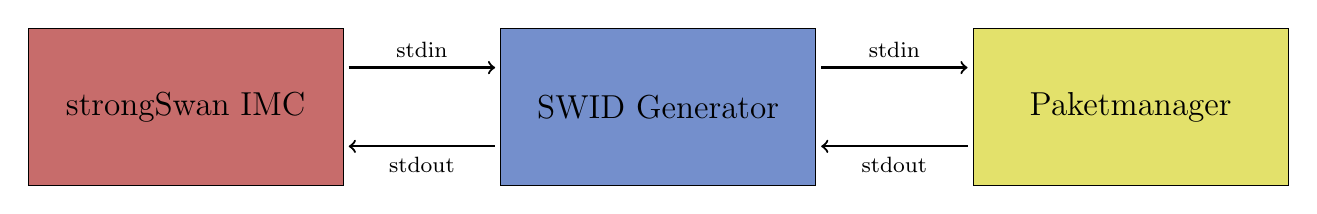
\begin{tikzpicture}[
		actor/.style={font=\large},
		communication/.style={thick, shorten <= 2pt, shorten >= 2pt, font=\footnotesize}
	]

	% Rectangles
	\filldraw[fill=StrongswanColor] (0, 0) rectangle node[actor] {strongSwan IMC} (4, 2);
	\filldraw[fill=GeneratorColor] (6, 0) rectangle node[actor] {SWID Generator} (10, 2);
	\filldraw[fill=PkgMgrColor] (12, 0) rectangle node[actor] {Paketmanager} (16, 2);

	% Arrows
	\draw[->, communication] (4, 1.5) -- node[above] {stdin} (6, 1.5);
	\draw[<-, communication] (4, 0.5) -- node[below] {stdout} (6, 0.5);
	\draw[->, communication] (10, 1.5) -- node[above] {stdin} (12, 1.5);
	\draw[<-, communication] (10, 0.5) -- node[below] {stdout} (12, 0.5);


\end{tikzpicture}

	\caption{SWID Generator: Systemkomponenten}
	\label{img:swid-generator-aktoren}
\end{figure}

\subsubsection{UC01: Erkennung des Paketmanagers}

\begin{usecase}
\hline
\textbf{Akteur} & strongSwan IMC \\
\hline
\textbf{Story} &
Der Akteur weiss nicht, welcher Paketmanager auf dem Zielsystem verwendet wird.
Der SWID Generator soll den verwendeten Paketmanager automatisch erkennen. \\
\hline
\textbf{Standard Szenario} &
Der SWID Generator erkennt den System-Paketmanager automatisch. \\
\hline
\textbf{Alternatives Szenario} &
Mittels optionalem Parameter kann der zu verwendende Paketmanager definiert
werden, die automatische Erkennung wird in diesem Fall nicht durchgeführt. \\
\hline
\end{usecase}


\subsubsection{UC02: Software ID Generierung}

\begin{usecase}
\hline
\textbf{Akteur} & strongSwan IMC \\
\hline
\textbf{Story} &
Der Akteur will die Software IDs aller installierten Pakete generieren. Das Format
dieser IDs folgt dem ISO Draft 19770-2\cite{iso19770-2} und besteht
aus der Regid des Tag Creators sowie der Unique ID des Tags. \\
\hline
\textbf{Standard Szenario} &
Alle Software IDs werden generiert und auf der Standardausgabe durch Newlines
(\texttt{\textbackslash{n}}) getrennt ausgegeben. Es wird eine Software ID pro Zeile
dargestellt. \\
\hline
\textbf{Alternatives Szenario} &
Die Trennzeichen zur Ausgabe der Software IDs können mittels optionalem
Parameter definiert werden. \\
\hline
\end{usecase}


\subsubsection{UC03: SWID Tag Generierung}

\begin{usecase}
\hline
\textbf{Akteur} & strongSwan IMC \\
\hline
\textbf{Story} &
Der Akteur will SWID Tags aller installierten Pakete generieren. Das Format
dieser XML Dokumente folgt dem ISO Draft 19770-2\cite{iso19770-2}. Für jedes
installierte Paket wird ein eigenes XML Dokument generiert. \\
\hline
\textbf{Standard Szenario} &
Alle Tags werden generiert und auf der Standardausgabe durch Newlines
(\texttt{\textbackslash{n}}) getrennt ausgegeben. Es wird ein Tag pro Zeile
dargestellt. Die Attribute des Tag Creators werden mit vordefinierten Werten
befüllt. Es ist ein definiertes Set Elemente und Attribute enthalten. \\
\hline
\textbf{Alternatives Szenario 1} &
Die Attribute des Tag Creators können mittels optionalen Parametern spezifiziert
werden. \\
\hline
\textbf{Alternatives Szenario 2} &
Die Trennzeichen zur Ausgabe der Tags können mittels optionalem Parameter
spezifiziert werden. \\
\hline
\textbf{Alternatives Szenario 3} &
Zu Debug-Zwecken können die Tags mittels optionalem Parameter in einer
eingerückten und einfacher lesbaren Form ausgegeben werden (\enquote{pretty
printing}). \\
\hline
\textbf{Alternatives Szenario 4} &
Mittels optionalem Parameter können die XML Tags mit einem Payload-Element
versehen werden, welches für jedes Paket die darin enthaltenen Dateien
auflistet. \\
\hline
\end{usecase}


\subsubsection{UC04: Targeted Request}
\label{swidgenerator:UC04}

\begin{usecase}
\hline
\textbf{Akteur} & strongSwan IMC \\
\hline
\textbf{Story} &
Der Akteur möchte nur den SWID Tag eines bestimmten Paketes erhalten. \\
\hline
\textbf{Standard Szenario} &
Mittels Parameter kann dem Generator ein Filterwert mitgegeben werden,
um einen bestimmten Tag herauszufiltern. Als Filterwert gibt es zwei Varianten:
Entweder den Package Name oder die Software ID. \\
\hline
\textbf{Alternatives Szenario 1} &
Die Attribute des Tag Creators können mittels optionalen Parametern spezifiziert
werden. \\
\hline
\textbf{Alternatives Szenario 2} &
Zu Debug-Zwecken können die Tags mittels optionalem Parameter in einer
eingerückten und einfach lesbaren Form ausgegeben werden (\enquote{pretty
printing}). \\
\hline
\textbf{Alternatives Szenario 3} &
Mittels optionalem Parameter können die XML Tags mit einem Payload-Element
versehen werden, welches für jedes Paket die darin enthaltenen Dateien
auflistet. \\
\hline
\end{usecase}

% }}}

% {{{ Paketmanager -----------------------------------------------------------%

\section{Paketmanager}
\label{swidgenerator:paketmanager}

Im Rahmen dieser Arbeit wurde die Unterstützung für drei der am weitesten
verbreiteten Paketverwaltungssysteme (DPKG, RPM und Pacman) implementiert. Damit
werden acht der zehn führenden Linux- und BSD-Distributionen gemäss
\enquote{DistroWatch.com}\cite{distrowatch:2014} abgedeckt.

Ein Paketmanager verwaltet unter anderem alle verfügbaren und installierten
Softwarepakete inklusive Meta-Informationen wie Paketname, Version oder
Installationsstatus.

\subsection{DPKG}

DPKG\footnote{\url{https://alioth.debian.org/projects/dpkg}} (Abkürzung für
\textit{Debian Package}) ist die Basis der Paketverwaltung in Debian und in
verwandten Distributionen wie Ubuntu.

\textbf{Liste installierter Pakete abfragen}

\begin{bashcode}
dpkg-query --show --showformat='${Package}\t${Version}\t${Status}\n'
\end{bashcode}

\textbf{Dateien zu Paket abfragen}

\begin{bashcode}
dpkg-query --listfiles <package-name>
\end{bashcode}

\textbf{Bemerkungen}

Entfernte DPKG Pakete können einen sogenannten \texttt{RC} Status haben. Dieser liegt
vor, wenn ein Paket deinstalliert wurde, aber die Konfigurationsdateien auf dem
System belassen wurden. Die \texttt{---show} Option liefert auch diese Pakete.
Der Status ist in der Ausgabe als \texttt{"deinstall ok config-files"}
ersichtlich, diese Pakete können so nachträglich herausgefiltert werden.


\subsection{RPM}

RPM\footnote{\url{https://rpm.org}} (Abkürzung für \textit{Red Hat Package
Manager}) ist der Standard-Paketmanager für Red Hat Linux Systeme sowie
verwandte Distributionen wie openSUSE, CentOS, Mandriva und Fedora.

\textbf{Liste installierter Pakete abfragen}

\begin{bashcode}
rpm -qa --queryformat %{name}\t%{version}-%{release}
\end{bashcode}

\textbf{Dateien zu Paket abfragen}

\begin{bashcode}
rpm -ql <package-name>
\end{bashcode}


\subsection{Pacman}

Pacman\footnote{\url{https://www.archlinux.org/pacman/}} ist der Paketmanager
unter Arch Linux und allen Derivaten wie Manjaro Linux oder Chakra.

\textbf{Liste installierter Pakete abfragen}

\begin{bashcode}
pacman -Q --color never
\end{bashcode}

\textbf{Dateien zu Paket abfragen}

\begin{bashcode}
pacman -Ql <package-name>
\end{bashcode}

% }}}

% {{{ Architektur ------------------------------------------------------------%

\section{Architektur}

\subsection{Übersicht}

Der SWID Generator wurde komplett in Python geschrieben und nutzt keine externen
Libraries. Es wird sowohl Python 2 wie auch Python 3 unterstützt.

Der Quellcode ist modular aufgebaut, gewisse Komponenten wurden in separate
Subpackages aufgeteilt:

\begin{figure}[H]
	\centering
	\definecolor{GeneratorColor}{RGB}{116,143,204}
\definecolor{GeneratorColorLight}{RGB}{195,206,230}

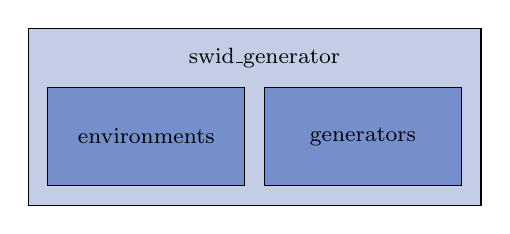
\begin{tikzpicture}[
		package/.style={fill=GeneratorColorLight},
		subpackage/.style={fill=GeneratorColor},
		every node/.style={font=\footnotesize}
	]

	% Packages
	\filldraw[package] (0, 0) rectangle  (5.75, 2.25);

	% Subackages
	\filldraw[subpackage] (0.25, 0.25) rectangle node {environments} (2.75, 1.5);
	\filldraw[subpackage] (3, 0.25) rectangle node {generators} (5.5, 1.5);

	% Labels
	\draw (3, 1.875) node {swid\_generator};

\end{tikzpicture}

	\caption{Aufteilung SWID Generator in Python Packages}
\end{figure}

Das Hauptpackage -- \texttt{swid\_generator} -- enthält folgende Module:

\begin{itemize}
	\item \texttt{main.py}: Der Einstiegspunkt in das Programm
	\item \texttt{argparser.py}: Klassen und Funktionen um
		Kommandozeilenargumente zu parsen
	\item \texttt{print\_functions.py}: Funktionen um Tag- und
		Software-ID-Generatoren auf die Standardausgabe auszugeben
	\item \texttt{package\_info.py}: DTO\footnote{Data Transfer Object, eine
		Klasse die kein Eigenverhalten aufweist sondern lediglich Daten in
		einem Objekt bündelt.}-Klassen für Dateien und Softwarepakete
	\item \texttt{exceptions.py}: Eigene Fehlerklassen
	\item \texttt{settings.py}: Globale Variablen, wie \zb
		\texttt{DEFAULT\_ENTITY\_NAME}
	\item \texttt{meta.py}: Metainformationen zum Generator, wie \zb der
		Programmname, die Lizenz oder die Version
\end{itemize}

Die zwei Subpackages sind für Input respektive Output zuständig. Im
\texttt{environments} Package sind die Environment-Klassen für die verschiedenen
Paketmanager enthalten. Die Klassen greifen auf die jeweiligen Paketdatenbanken
zu und geben diese Informationen an das Hauptprogramm zurück. Die
Environment-Registry befindet sich ebenfalls in diesem Package. Mehr dazu im
Abschnitt \ref{swidgenerator:architektur:environments}. Das \texttt{generators}
Package enthält die nötigen Funktionen, um aus den durch das entsprechende
Environment zurückgegebenen Paketinformationen, die dazugehörigen Software IDs
oder SWID Tags zu generieren. Mehr dazu im Abschnitt
\ref{swidgenerator:architektur:generatoren}.

Als Einstiegspunkt in den SWID Generator dient das \texttt{main.py} Modul. Um
das Programm direkt aus dem Quellcode-Ordner heraus zu starten, sollte Python
mit der \texttt{-m} Option und dem vollständigen Modulpfad gestartet werden:

\begin{bashcode}
python -m swid_generator.main
\end{bashcode}

Wenn das Programm über \texttt{pip} oder \texttt{setup.py} installiert wird (siehe
\autoref{swidgenerator:architektur:deployment}), kann es natürlich auch direkt
über den Programmnamen aufgerufen werden:

\begin{bashcode}
swid_generator
\end{bashcode}

\subsection{Ablauf}

\subsubsection{Initialisierung}
\label{swidgenerator:architektur:initialisierung}

Wenn der SWID Generator gestartet wird, beginnt die Code-Ausführung im
\texttt{main.py} Modul. Zuerst müssen die modular aufgebauten
Environment-Klassen registriert werden. Danach werden alle
Kommandozeilen-Argumente verarbeitet. Mit den nun vorhandenen Informationen muss
entschieden werden, welches Environment effektiv verwendet werden soll --
entweder durch den Benutzer definiert oder durch die automatische
Paketmanager-Erkennung.

Der Ablauf ist wie folgt:

\begin{enumerate}
	\item Die Environment Registry
		(Abschnitt \ref{swidgenerator:architektur:environments:registry}) wird initialisiert.
	\item Alle verfügbaren Environment Klassen
		(Abschnitt \ref{swidgenerator:architektur:environments}) werden der Registry
		übergeben.
	\item Der Argument Parser wird mit einer Referenz auf die Registry instanziert.
	\item Die Parser Instanz parst mithilfe des \texttt{argparse} Moduls aus der
		Python Stanardbibliothek die Kommandozeilen-Argument und generiert daraus ein
		\enquote{Options}-Objekt. \item Dieses Objekt wird nun der Environment Registry
		übergeben. Diese kann mit den Informationen darin die geeignete Environment
		Klasse finden und an das Hauptprogramm zurückgeben. Das Environment kann per
		Kommandozeilen-Argument vorgegeben werden, andernfalls wird es automatisch
		detektiert.
\end{enumerate}

In der folgenden Abbildung ist dieser Ablauf als UML Sequenzdiagramm
dargestellt:

\begin{figure}[H]
	\centering
	\begin{tikzpicture}
	\begin{umlseqdiag}[font=\footnotesize]

		% Objekte

		\umlobject{main}
		\umlcreatecall[dt=5, x=8, class=EnvironmentRegistry]{main}{registry}

		% Calls

		\begin{umlfragment}[type=loop, label=foreach env, inner xsep=10]
			\begin{umlcall}[dt=7, padding=2, op={register(env)}]{main}{registry}
			\end{umlcall}
		\end{umlfragment}

		\umlcreatecall[dt=7, x=4, class=MainArgumentParser]{main}{parser}
		\begin{umlcall}[dt=3, padding=4, op={parse(registry)},return=options]{main}{parser}
		\end{umlcall}

		\begin{umlcall}[dt=7, padding=3, op={get\_environment(options)},return=env]{main}{registry}
			\begin{umlfragment}[type=opt, label=if !options.env, inner xsep=15]
				\begin{umlcallself}[op=autodetect\_env()]{registry}
				\end{umlcallself}
			\end{umlfragment}
		\end{umlcall}

	\end{umlseqdiag}
\end{tikzpicture}

	\caption{Sequenzdiagramm, Initialisierung}
\end{figure}

\subsubsection{Generierung}
\label{swidgenerator:architektur:generierung}

Nachdem nun, wie im Abschnitt \ref{swidgenerator:architektur:initialisierung}
beschrieben, alle nötigen Informationen gesammelt wurden, kann nun die
Hauptarbeit geschehen: die Generierung der Daten aus den
Paketmanager-Informationen. Ob SWID Tags oder Software-IDs generiert werden, ist
abhängig vom ersten Kommandozeilenargument, welches entweder \texttt{swid} oder
\texttt{software-id} sein kann.

\begin{enumerate}
	\item Zuerst werden mithilfe des SWID Tag Generators (Abschnitt
	\ref{swidgenerator:architektur:generatoren}) die benötigten Informationen aus
	der Paketmanager-Datenbank ausgelesen und daraus SWID Tags generiert.
		
	\item Die zurückgegebenen Tags werden mit Hilfe der entsprechenden
	Print-Funktionen (Abschnitt \ref{swidgenerator:architektur:printers}) auf die
	Standardausgabe ausgegeben.
		
	\item Falls im ganzen Programmablauf keine Fehler aufgetreten sind, wird das
	Programm nun mit dem Status Code 0 (=keine Fehler) beendet.
\end{enumerate}

Dieser Ablauf ist im folgenden UML Sequenzdiagramm visualisiert:

\begin{figure}[H]
	\centering
	\begin{tikzpicture}
	\begin{umlseqdiag}

		% Objekte

		\umlobject[x=0]{main}
		\umlobject[x=4]{generator}
		\umlobject[x=6.5]{printer}
		\umlobject[x=9]{sys}

		% Calls

		\begin{umlfragment}[type=alt, label={command = "{}swid"}, inner xsep=23, inner ysep=2]

			\begin{umlcall}[padding=4, dt=10, op=create\_swid\_tags(), return=tags]{main}{generator}
			\end{umlcall}
			\begin{umlcall}[dt=6, op=print\_swid\_tags(tags), return={\ }]{main}{printer}
			\end{umlcall}

			\umlfpart[command = "{}software-id"]

			\begin{umlcall}[padding=4, op=create\_software\_ids(), return=ids]{main}{generator}
			\end{umlcall}
			\begin{umlcall}[dt=0, op=print\_software\_ids(ids), return={\ }]{main}{printer}
			\end{umlcall}

		\end{umlfragment}

		\begin{umlcall}[dt=2, op=exit(0)]{main}{sys}
		\end{umlcall}

	\end{umlseqdiag}
\end{tikzpicture}

	\caption{Sequenzdiagramm, Generierung}
\end{figure}


\subsection{Implementationsdetails}

\subsubsection{Environments}
\label{swidgenerator:architektur:environments}

Die Environments sind das Kernstück des SWID Generators, sie greifen auf
den System-Paketmanager zu und bereiten die Liste der installierten Pakete für
die weitere Verarbeitung auf.

Wie bereits im Abschnitt \ref{swidgenerator:paketmanager} erwähnt, bietet der
SWID Generator zum aktuellen Zeitpunkt Unterstützung für drei Paketmanager an.
Damit der SWID Generator in Zukunft auch auf bisher noch nicht unterstützten
Systemen wie Slackware Linux, FreeBSD oder Windows einsatzfähig ist, wurde Wert
darauf gelegt, dass sich das Hinzugfügen neuer Environments einfach gestaltet.

Um dieses Ziel zu erreichen, ist eine einheitliche Schnittstelle für die
Environment-Klassen essentiell. Wie es in Python üblich
ist\cite{contracts:2003}, wird dafür ein Ansatz mit impliziten Contracts
anstelle von explizit ausprogrammierten Interfaces verwendet. Dieser
Architektur-Ansatz ist auch als \textit{Duck Typing} bekannt.

Damit eine Klasse ein gültiges Environment darstellt, benötigt sie die folgenden
fünf Methoden:

\begin{itemize}
	\item \texttt{get\_package\_list()}: Gibt eine Liste von
		\texttt{swid\_generator.\-package\_info.\-PackageInfo} Instanzen zurück,
		welche die installierten Softwarepakete auf dem aktuellen System
		repräsentiert.
	\item \texttt{get\_files\_for\_package(package\_name)}: Akzeptiert einen
		Paketnamen und gibt eine Liste von
		\texttt{swid\_generator.\-package\_info.\-FileInfo}-Instanzen zurück, welche
		die zu einem Softwarepaket gehörigen Dateien repräsentiert.
	\item \texttt{is\_installed()}: Prüft, ob der repräsentierte Paketmanager auf
		dem aktuellen System installiert ist oder nicht. Dies kann beispielseweise
		getan werden, indem geprüft wird, ob zentrale Executables (\zb
		\texttt{dpkg-query} bei DPKG) vorhanden sind.
	\item \texttt{get\_architecture()}: Gibt den System-Architekturtyp (\zb
		\texttt{x86\_64} oder \texttt{i386}) zurück.
	\item \texttt{get\_os\_string()}: Gibt den Bezeichner der aktuellen
		Betriebssystem-Distribution zurück (\zb \texttt{debian\_7.4} oder
		\texttt{fedora\_19}).
\end{itemize}

Da Environments meist gemeinsam benötigte Funktionalität aufweisen --
beispielsweise die Überprüfung, ob eine vom Paketmanager gemeldete Datei auch
wirklich auf dem System vorhanden ist -- wurden diese in eine Basisklasse namens
\texttt{CommonEnvironment} ausgegliedert. Diese kann wahlweise von einem
Environment erweitert werden.

Die aktuell vorhandenen Environment-Klassen sind folgendermassen organisiert:

\begin{figure}[H]
	\centering
	\resizebox{\textwidth}{!}{%
		\begin{tikzpicture}

	\begin{umlpackage}{environments}[font=\sffamily]

		\umlclass[x=5.5, y=4]{CommonEnvironment}{}{
			get\_architecture() \\
			get\_os\_string() \\
			is\_installed() \\
			\_is\_file(path)
		}

		\umlclass[x=0, y=0]{DpkgEnvironment}{}{
			get\_package\_list() \\
			get\_files\_for\_package(name) \\
			\_package\_installed(package)
		}
		\umlinherit{DpkgEnvironment}{CommonEnvironment}

		\umlclass[x=5.5, y=0.25]{RpmEnvironment}{}{
			get\_package\_list() \\
			get\_files\_for\_package(name)
		}
		\umlinherit{RpmEnvironment}{CommonEnvironment}

		\umlclass[x=11, y=0.25]{PacmanEnvironment}{}{
			get\_package\_list() \\
			get\_files\_for\_package(name)
		}
		\umlinherit{PacmanEnvironment}{CommonEnvironment}

	\end{umlpackage}

\end{tikzpicture}

	}
	\caption{Die Environment-Klassen}
	\label{img:environment-klassendiagramm}
\end{figure}


\subsubsection{Die Registry}
\label{swidgenerator:architektur:environments:registry}

Nachdem eine Environment-Klasse definiert wurde (siehe Abschnitt
\ref{swidgenerator:architektur:environments}), muss diese im Hauptprogramm
registriert und verwaltet werden. Dies ist die Aufgabe der
\texttt{EnvironmentRegistry}-Klasse.

Das Kernstück dieser Klasse ist die \texttt{register()}-Funktion. Sie benötigt als
Argumente eine Kurzbezeichnung für das Environment sowie eine Referenz auf die
Environment-Klasse. Beispiel:
\begin{listing}[H]
\caption{Registrieren von Environments}
\begin{pythoncode}
registry = EnvironmentRegistry()
registry.register('rpm', RpmEnvironment)
registry.register('dpkg', DpkgEnvironment)
registry.register('pacman', PacmanEnvironment)
\end{pythoncode}
\end{listing}

Die Klassen werden als Instanzen intern in einem Dictionary gespeichert. Um die
Liste der verfügbaren Environments abzufragen, kann die
\texttt{get\_environment\_strings()} Methode verwendet werden:

\begin{listing}[H]
\caption{Verfügbare Environments abfragen}
\begin{pythoncode}
>>> registry.get_environment_strings()
['auto', 'dpkg', 'pacman', 'rpm']
\end{pythoncode}
\end{listing}

Als Resultat werden die Kurzbezeichnungen der registrierten Environments
alphabetisch sortiert aufgelistet. Zusätzlich wird der String \texttt{'auto'}
zurückgeliefert, welcher für die automatische Environment Erkennung steht. Diese
Liste wird vom Argument Parser verwendet, um die Liste der gültigen Werte für die
\texttt{-{}-env} Option zu finden.

Die dritte wichtige Methode der \texttt{EnvironmentRegistry}-Klasse ist
\texttt{get\_environment()}. Diese nimmt eine Environment-Kurzbezeichnung
entgegen und führt folgende Schritte aus:

\begin{enumerate}
	\item Wenn die Kurzbezeichnung \texttt{'auto'} ist, wird versucht, das
	installierte Environment automatisch zu finden, indem über die Liste der
	registrierten Environments iteriert wird und für jedes Environment geprüft
	wird, ob der passende Paketmanager auf dem System installiert ist. Das erste
	Environment, bei dem dies zutrifft, wird zurückgegeben. Falls dies für keines
	der Environments der Fall sein sollte, wird eine \texttt{AutodetectionError}
	Exception ausgelöst.
	
	\item Wenn die Kurzbeschreibung nicht \texttt{'auto'} ist, wird die passende
	Environment Instanz aus dem internen Dictionary geholt. Wenn keine
	entsprechende Instanz gefunden wird, wird ein \texttt{KeyError} ausgelöst.
		
	\item Zuletzt wird geprüft, ob das zurückgegebene Environment installiert
	ist. Wenn nicht, wird eine \texttt{EnvironmentNotInstalledError} Exception
	ausgelöst. Ansonsten wird die Environment-Instanz zurückgegeben.
\end{enumerate}

\subsubsection{Generatoren}
\label{swidgenerator:architektur:generatoren}

Die Generatoren im \texttt{generators} Package sind dafür zuständig, aus den
durch das entsprechende Environment zurückgegebenen Paketinformationen die
dazugehörigen Software-IDs oder SWID Tags zu generieren.

Diese Funktionen sind als Python Generator-Funktionen\cite[S.~94-95]{alchin2010pro}
implementiert und geben die einzelnen Resultat-Strings mit \texttt{yield}
anstelle von \texttt{return} zurück. Dadurch kann über alle SWID Tags oder über
alle Software-IDs iteriert werden, ohne dass alle Strings gleichzeitig in den
Hauptspeicher geladen werden müssen. Jedes Mal wenn auf der Generator-Instanz
\texttt{next()} aufgerufen wird, wird nur der nächste String berechnet. Dieses
Prinzip ist auch als \enquote{Lazy Evaluation}\cite[S.~85--93]{meyers1995more}
bekannt.

\subsubsection{Print-Funktionen}
\label{swidgenerator:architektur:printers}

Die Print-Funktionen sind im Modul \texttt{print\_functions.py} enthalten. Ihre
Aufgabe ist es, den Output der Generatoren korrekt auf die Standardausgabe zu
schreiben.

Aktuell sind zwei Print-Funktionen definiert, eine für die SWID Tags und eine
für die Software-IDs. Beide nehmen einen Generator entgegen und geben den Inhalt
Zeile für Zeile aus, getrennt durch ein vordefiniertes Trennzeichen.

Die Art, wie die Inhalte ausgegeben werden, ist jedoch unterschiedlich. Während
die XML Tags normal oder in einer \enquote{prettified} Version ausgegeben werden
können, werden die Software-IDs direkt ausgegeben, ohne sie zu manipulieren. Aus
diesem Grund haben wir für die Implementierung das Strategy
Pattern\cite{gamma1994design} verwendet.

Es gibt eine generische Funktion namens \texttt{iterate}, welche als Argumente
den Generator, eine Action-Funktion (die \enquote{Strategie}), einen Separator
und einen End-String annimmt. Die Funktionsimplementation sieht folgendermassen
aus:

\begin{listing}[H]
\caption{Implementation der Iterate-Funktion}
\begin{pythoncode}
def iterate(generator, action_func, separator, end):
    item = next(generator)
    while item:
        action_func(item)
        try:
            item = next(generator)
            safe_print(separator, end='')
        except StopIteration:
            safe_print(end, end='')
            break
\end{pythoncode}
\end{listing}

Die einfachste Form eines Aufrufes wird für die Software-IDs verwendet, wo die
Action-Funktion keine weitere Logik enthält als die Ausgabe des Strings (siehe
Listing \ref{swidgenerator:architektur:software-id-print}). Die SWID-Tag Version
sieht ähnlich aus, allerdings wird dort zusätzlich das \enquote{Prettifying} der
XML Tags durchgeführt.

\begin{listing}[H]
\caption{Implementation der Software-ID Print-Funktion}
\label{swidgenerator:architektur:software-id-print}
\begin{pythoncode}
def action(swid):
    safe_print(swid, end='')
iterate(software_ids, action, separator, end='\n')
\end{pythoncode}
\end{listing}

% TODO: Ev Sequenzdiagramm?

Dadurch, dass die Generatoren jeweils nur ein einzelnes Element zurückgeben,
kann dieses sofort auf die Standardausgabe geschrieben werden und dann vom
Garbace Collector gelöscht werden. Dies spart einerseits Arbeitsspeicher,
andererseits kann es die Wartezeit eines aufrufenden Programmes verkürzen, da es
mit der Verarbeitung bereits beginnen kann bevor alle Daten generiert und
ausgegeben worden sind.

\subsubsection{Python 3 Kompatibilität}

Obwohl Python 3.0 bereits im Jahr 2008 veröffentlicht wurde, hat es sich bisher
noch nicht durchgesetzt. Da mit dieser Version
die Rückwärtskompatibilität gebrochen wird, wehrten sich viele Entwickler
gegen einen Wechsel von der etablierten Version 2 auf Python 3. Einerseits
war es anfänglich schwierig, Python 2 und 3 mit einer einzigen Codebasis zu
unterstützen, andererseits nutzten viele Programme Dritt-Bibliotheken welche
noch nicht auf Python 3 portiert waren.

Seit mit Python 3.3 der Unicode-Präfix für Strings wieder eingeführt
wurde\cite{PEP414:2012}, ist die Unterstützung beider Sprachversionen mit einer
einzigen Codebasis jedoch bedeutend einfacher geworden. Auch wurden mehrere
Portierungs-Ratgeber publiziert, welche die Übergangsphase
vereinfachen\cite{regebro2013porting, ronacher2013porting}. Die Adoptionsrate
stieg dadurch stark an, so dass inzwischen 162 der 200 meistgenutzten Python
Pakete mit Python 3 kompatibel sind\cite{py3adoption}.

Bei der Entwicklung wurden vor allem die Hinweise aus dem Ratgeber
\enquote{Quick Tips on Making Your Code Python 3 Ready}\cite{deshev2012porting}
verwendet. Eines der wichtigsten Elemente daraus ist der folgende
\enquote{Future-Header}:

\begin{pythoncode}
from __future__ import print_function, division, absolute_import, unicode_literals
\end{pythoncode}

Durch die konsequente Nutzung dieser Import-Zeile in jedem Python-Modul konnten
die Inkompatibilitäten stark reduziert werden; die Portierung auf Python 3.3 und
3.4 war anschliessend einfach umzusetzen.

Um die Ausgabe von Unicode- wie auch Byte-Strings unter beiden Versionen zu
vereinfachen, haben wir zusätzlich eine \texttt{safe\_print} Funktion definiert
(Listing \ref{safeprint}).

\begin{listing}[h]
\caption{Safe-Print Funktion}
\label{safeprint}
\begin{pythoncode}
def safe_print(data, end='\n'):
    # Python 3
    if hasattr(sys.stdout, 'buffer'):
        if isinstance(data, bytes):
            sys.stdout.buffer.write(data)
        else:
            sys.stdout.write(data)
        if isinstance(end, bytes):
            sys.stdout.buffer.write(end)
        else:
            sys.stdout.write(end)
        sys.stdout.flush()
    # Python 2
    else:
        print(data, end=end)
\end{pythoncode}
\end{listing}

Zur Sicherstellung der Kompatibilität wurde die Test Suite zudem so
konfiguriert, dass die Tests auf allen unterstützten Python-Versionen ausgeführt
werden (Abschnitt \ref{swidgenerator:architektur:qa}).
% }}}

% {{{ Ergebnisse -------------------------------------------------------------%

\section{Ergebnisse}

\subsection{Generieren von Software IDs}

Der SWID Generator kann folgendermassen verwendet werden, um Software-IDs zu
generieren:

\begin{listing}[H]
\caption{Generierung von Software-IDs}
\begin{textcode}
usage: swid_generator software-id [-h] [--env {auto,dpkg,pacman,rpm}]
                                  [--doc-separator DOCUMENT_SEPARATOR]
                                  [--regid REGID]
\end{textcode}
\end{listing}

Nachfolgend ein Beispielaufruf auf einem Debian-System:

\begin{listing}[H]
\caption{Software-ID Auszug eines Debian-Systems}
\begin{textcode}
$ swid_generator software-id --regid=regid.1998-05.ch.hsr
regid.1998-05.ch.hsr_debian_7.4-x86_64-acpi-1.6-1
regid.1998-05.ch.hsr_debian_7.4-x86_64-acpi-support-base-0.140-5
...
regid.1998-05.ch.hsr_debian_7.4-x86_64-zlib1g-1:1.2.7.dfsg-13
regid.1998-05.ch.hsr_debian_7.4-x86_64-zlib1g-dev-1:1.2.7.dfsg-13
\end{textcode}
\end{listing}

Die vollständige Dokumentation der Optionen kann auf der Kommandozeile mit dem
\texttt{-{}-help} Parameter ausgegeben werden.


\subsection{Generieren von SWID Tags}

Die Syntax um SWID Tags zu generieren sieht folgendermassen aus:

\begin{listing}[H]
\caption{Generieren von SWID Tags}
\begin{textcode}
usage: swid_generator swid [-h] [--env {auto,dpkg,pacman,rpm}]
                           [--doc-separator DOCUMENT_SEPARATOR]
                           [--regid REGID] [--entity-name ENTITY_NAME]
                           [--full] [--pretty]
                           [--software-id SOFTWARE-ID | --package PACKAGE]
\end{textcode}
\end{listing}

Hier ein Beispiel eines Targeted Requests für das \texttt{cowsay}-Paket mit
\enquote{Pretty-Printing}:

\begin{listing}[H]
\caption{Beispiel eines Targeted Requests}
\begin{xmlcode}
$ swid_generator swid --package cowsay --pretty
<?xml version="1.0" encoding="utf-8"?>
<SoftwareIdentity name="cowsay" uniqueId="debian_7.4-x86_64-cowsay-3.03+dfsg1-4"
      version="3.03+dfsg1-4" versionScheme="alphanumeric"
      xmlns="http://standards.iso.org/iso/19770/-2/2014/schema.xsd">
  <Entity name="strongSwan" regid="regid.2004-03.org.strongswan" role="tagcreator"/>
</SoftwareIdentity>
\end{xmlcode}
\end{listing}


\subsection{Performance}

Durch die in den Abschnitten \ref{swidgenerator:architektur:generatoren} und
\ref{swidgenerator:architektur:printers} beschriebenen Optimierungen konnte die
Ausgabe des SWID Generators beschleunigt werden. Nachfolgend ein paar
Geschwindigkeitsmessungen, die auf verschiedenen Systemen durchgeführt wurden.
Getestet wurden dabei die folgenden Befehle:

\begin{itemize}
	\item ids: \texttt{swid\_generator software-id > /dev/null}
	\item tags: \texttt{swid\_generator swid > /dev/null}
	\item tags-full: \texttt{swid\_generator swid -{}-full > /dev/null}
	\item tags-full-pretty: \texttt{swid\_generator swid -{}-pretty -{}-full > /dev/null}
\end{itemize}

Die Befehle wurden jeweils mehrmals ausgeführt, um mögliche Caching-Effekte
auszugleichen. Nachfolgend die getesteten Systeme:

\begin{itemize}
	\item dpkg-952: DPKG, 952 installierte Pakete
	\item pacman-1223: Pacman, 1223 installierte Pakete
	\item rpm-437: RPM, 437 installierte Pakete
\end{itemize}

Die Ergebnisse:

\begin{tabularx}{\textwidth}{rCCC}
	& \textbf{dpkg-952} & \textbf{pacman-1223} & \textbf{rpm-437} \\
	\hline
	\textbf{ids} & 0.143s & 0.054s & 0.511s \\
	\hline
	\textbf{tags} & 0.227s & 0.102s & 0.534\\
	\hline
	\textbf{tags-full} & 34.256s & 13.822s & 6.213s \\
	\hline
	\textbf{tags-full-pretty} & 54.039s & 31.202s & 8.920s \\
	\hline
\end{tabularx}

\vspace{1.5em}

Da auf den Systemen nicht gleich viele und gleich grosse Pakete installiert
sind, sind diese Resultate schwer vergleichbar. Man kann jedoch die zu
erwartende Laufzeit abschätzen.

Klar ersichtlich ist, dass der grösste Zeitaufwand beim Generieren von SWID Tags
mit der \texttt{-{}-full} Option auftritt. Dies ist erklärbar, da hierbei jede
Datei in jedem installierten Paket auf dem System vom SWID Generator auf
Existenz geprüft wird. An diesem Punkt gibt es möglicherweise noch
Optimierungspotential.

Das Pretty Printing ist ebenfalls ein zeitaufwändiger Vorgang, da die
generierten Tags hierfür ein zweites Mal geparsed und in einer
\enquote{schöneren} Variante ausgegeben werden müssen. Der Mehraufwand gegenüber
der Variante ohne \texttt{-{}-pretty} betrug in den drei gemessenen
Beispielfällen zwischen 43\% und 125\%. Da diese Option nur für Debugging-Zwecke
gebraucht werden sollte, ist dies in der Praxis kein nenneswertes Problem und
auch kaum ein sinnvolles Ziel für Optimierungen.


% }}}

% {{{ Qualitätsmanagement ----------------------------------------------------%

\section{Qualitätsmanagement}
\label{swidgenerator:architektur:qa}

Wie es in Abschnitt \ref{improvements:tests} genauer erläutert wird, haben wir
zum Schreiben und Ausführen der Testsuite Pytest verwendet. Im Gegensatz zu
strongTNC muss der swidGenerator jedoch nicht nur eine Python-Version
unterstützen, sondern gleich mehrere, da die Deployment-Ziele (TNC Clients)
eine höhere Betriebssystem-Diversität aufweisen.

Um dies zu gewährleisten, wurde Tox\footnote{\url{http://tox.readthedocs.org/}}
verwendet. Tox ist ein Tool welches gemäss einer Konfigurationsdatei automatisch
verschiedene \enquote{Virtualenvs} erstellt. Jedes Virtualenv enthält eine
andere Python-Version mit den entsprechenden Abhängigkeiten. Die Testsuite wird
anschliessend in jedem Virtualenv separat ausgeführt.

\begin{figure}[H]
	\centering
	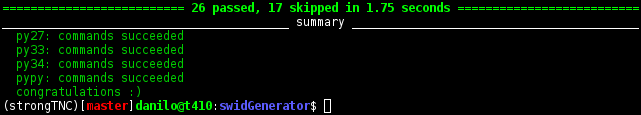
\includegraphics[width=0.8\textwidth]{images/tox-result}
	\caption{Tox Resultate}
	\label{swidgenerator:qa:tox}
\end{figure}

Wie im Abschnitt \ref{improvements:travis} beschrieben, wird auch für den SWID
Generator Travis CI eingesetzt. Mit der entsprechenden Konfiguration wird jede
von Tox unterstützte Version in einem separaten Job getestet. Die Resultate
werden dann als Build Matrix dargestellt.

\begin{figure}[H]
	\centering
	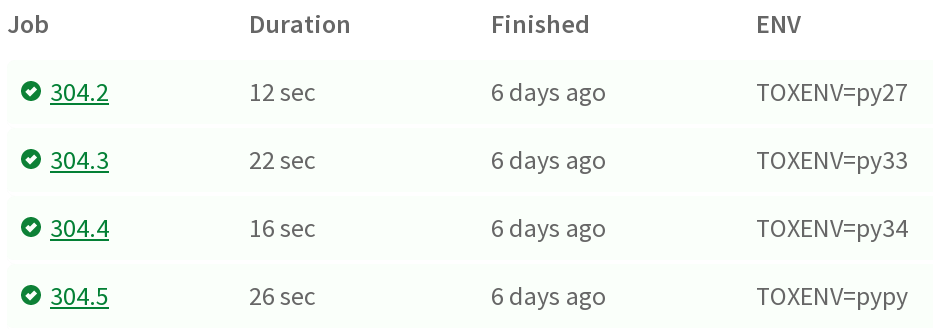
\includegraphics[width=0.6\textwidth]{images/travis-results}
	\caption{Tox Resultate}
	\label{swidgenerator:qa:tox}
\end{figure}

Wie auch bei strongTNC werden beim SWID Generator die Coding-Guidelines durch
die Test Suite forciert. Zuwiderhandlungen gegen die Guidelines werden als
Fehler betrachtet.

% }}}

% {{{ Packaging --------------------------------------------------------------%

\section{Packaging}
TODO Danilo
- Setup.py
- Manifest.in
- meta.py

% }}}

% {{{ Deployment -------------------------------------------------------------%

\section{Deployment}
\label{swidgenerator:architektur:deployment}
TODO Danilo

% }}}
